\chapter*{Apêndice 5: Banco de dados Neo4j}
\label{apendice:neo4j}

Neste Apêndice serão apresentados os passos para a instalação do banco de dados Neo4j.

\par Para realizar o \textit{download} do instalador do banco de dados Neo4j, deve-se acessar a seguinte URL, por meio de um  navegador de internet: http://neo4j.com/download e selecionar a opção desejada. Neste trabalho como já descrito foi utilizada a versão \textit{Community}. A Figura~\ref{fig:ap3:download_neo4j} apresenta a página de \textit{download} do Neo4j.

\captionsetup[figure]{list=no}
\begin{figure}[h!]
	\centerline{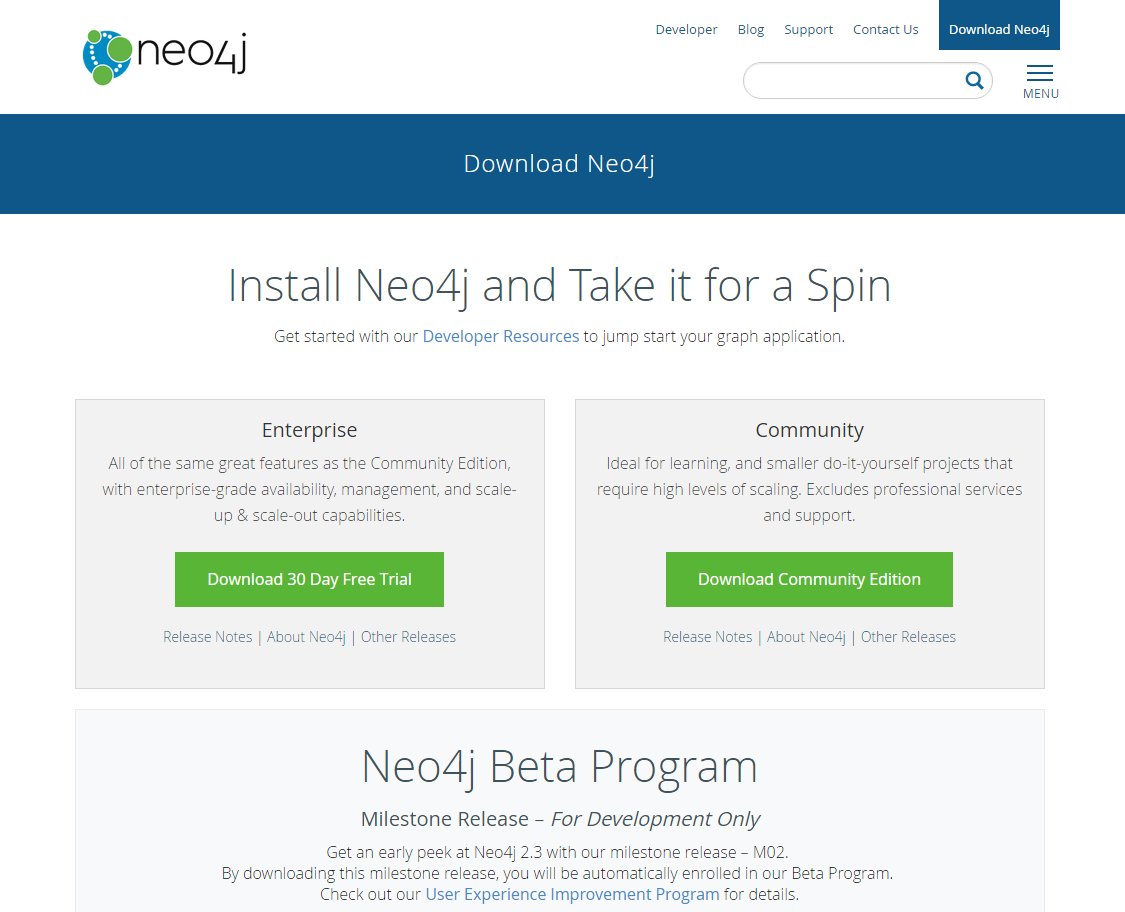
\includegraphics[scale=0.4]{./imagens/apendices/download-neo4j.png}}
	\caption[Página de \textit{download} do Neo4j]
	{Página de \textit{download} do Neo4j. \textbf{Fonte:} http://neo4j.com/download}
	\label{fig:ap3:download_neo4j}
\end{figure}

\par Após concluído o \textit{download}, deve-se executar o arquivo. O processo de instalação se inicia e a primeira tela apresentada ao usuário é a tela contendo uma mensagem de boas vindas, conforme demonstra a Figura~\ref{fig:ap3:boas_vindas_neo4j}. Nesta tela, deve-se clicar no botão \textit{Next} para prosseguir com o processo de instalação.

\newpage
\captionsetup[figure]{list=no}
\begin{figure}[h!]
	\centerline{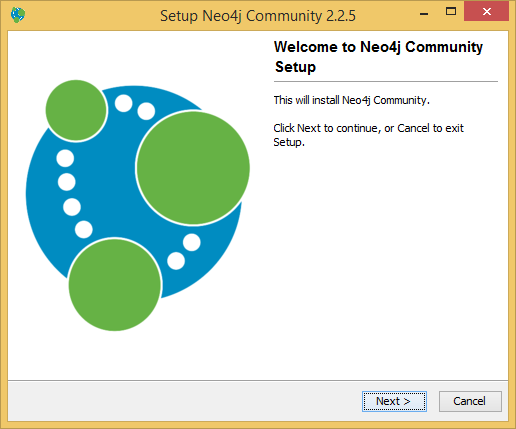
\includegraphics[scale=0.4]{./imagens/apendices/neo4j-install-step1.png}}
	\caption[Tela de boas vindas da instalação do Neo4j]
	{Tela de boas vindas da instalação do Neo4j. \textbf{Fonte:} Elaborado pelos autores.}
	\label{fig:ap3:boas_vindas_neo4j}
\end{figure}

\par A próxima tela apresentada ao usuário diz respeito ao contrato de uso do \textit{software}, como mostra a Figura~\ref{fig:ap3:contrato_neo4j}. Após lê-lo, deve-se aceitar os termos do contrato e clicar em \textit{Next}.

\captionsetup[figure]{list=no}
\begin{figure}[h!]
	\centerline{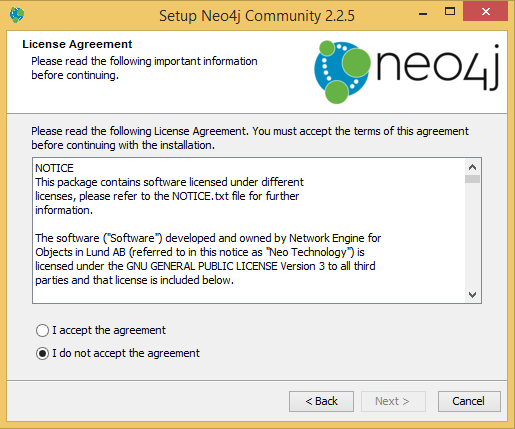
\includegraphics[scale=0.4]{./imagens/apendices/neo4j-install-step2.png}}
	\caption[Tela do contrato de uso do Neo4j]
	{Tela do contrato de uso do Neo4j. \textbf{Fonte:} Elaborado pelos autores.}
	\label{fig:ap3:contrato_neo4j}
\end{figure}

\par Na próxima tela, conforme a Figura~\ref{fig:ap3:definicao_diretorio_neo4j} demonstra, é definido o diretório de instalação do Neo4j. Por padrão este diretório é o mesmo das demais aplicações no \textit{Windows}, podendo ser alterado conforme a necessidade. Após definir o diretório de instalação deve-se clicar no botão \textit{Next}.

\captionsetup[figure]{list=no}
\begin{figure}[h!]
	\centerline{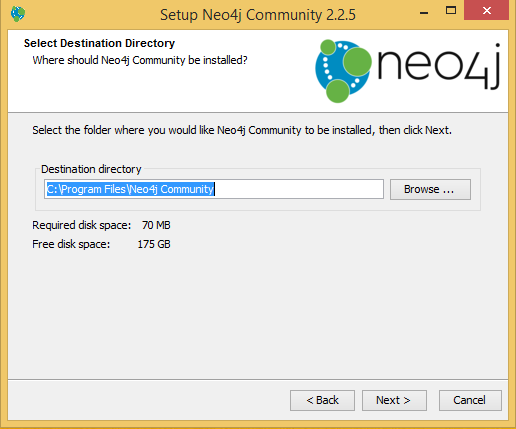
\includegraphics[scale=0.4]{./imagens/apendices/neo4j-install-step3.png}}
	\caption[Tela para definição do diretório de instalação do Neo4j]
	{Tela para definição do diretório de instalação do Neo4j. \textbf{Fonte:} Elaborado pelos autores.}
	\label{fig:ap3:definicao_diretorio_neo4j}
\end{figure}

\par Após as definições anteriores, uma tela é apresentada questionando o usuário a respeito da criação de atalhos na área de trabalho, como é demonstrado na Figura~\ref{fig:ap3:criacao_atalho_neo4j}. Posterior à definição dos atalhos do Neo4j, deve-se clicar no botão \textit{Next}.

\captionsetup[figure]{list=no}
\begin{figure}[h!]
	\centerline{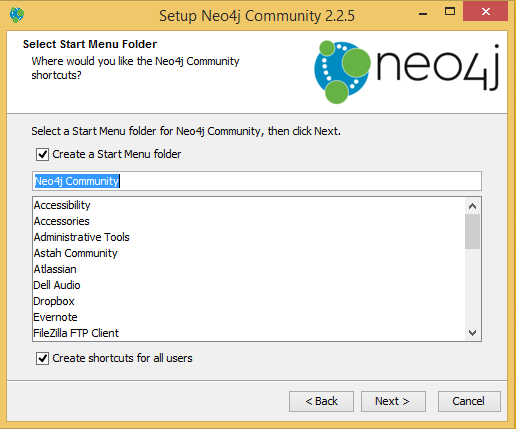
\includegraphics[scale=0.4]{./imagens/apendices/neo4j-install-step4.png}}
	\caption[Tela para criação de atalhos do Neo4j]
	{Tela para criação de atalhos do Neo4j. \textbf{Fonte:} Elaborado pelos autores.}
	\label{fig:ap3:criacao_atalho_neo4j}
\end{figure}

\par Após realizar os procedimentos descritos para a instalação do Neo4j a tela final de instalação será apresentada, informando-o a respeito do resultado da instalação conforme demonstra a Figura~\ref{fig:ap3:tela_final_neo4j}. Clique no botão \textit{Finish} para finalizar o processo de instalação.
Após todos os passos realizados com sucesso, o Neo4j estará disponível.

\captionsetup[figure]{list=no}
\begin{figure}[h!]
	\centerline{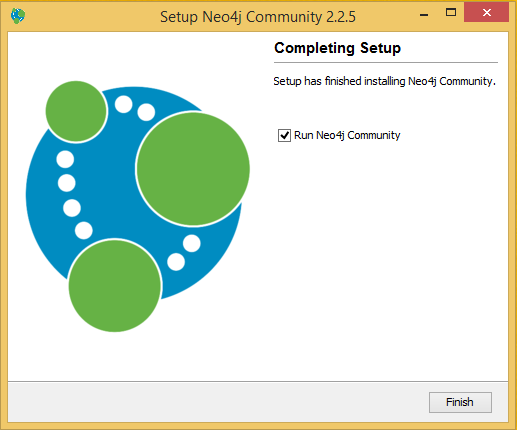
\includegraphics[scale=0.4]{./imagens/apendices/neo4j-install-step5.png}}
	\caption[Tela final de instalação do Neo4j]
	{Tela final de instalação do Neo4j. \textbf{Fonte:} Elaborado pelos autores.}
	\label{fig:ap3:tela_final_neo4j}
	
\end{figure}

\par A Figura~\ref{fig:ap3:tela_inicial_neo4j} apresenta a tela inicial do Neo4j após sua instalação. Para iniciar a utilização desse banco de dados, clique no botão \textit{"Start"}.

\captionsetup[figure]{list=no}
\begin{figure}[h!]
	\centerline{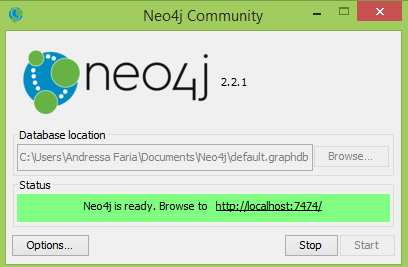
\includegraphics[scale=0.60]{./imagens/apendices/neo4j.jpg}}
	\caption[Tela de inicialização do Neo4j ]
	{Tela de inicialização do Neo4j \textbf{Fonte:} Elaborado pelos autores.}
	\label{fig:ap3:tela_inicial_neo4j}
\end{figure}

\par Após realizar todos os procedimentos descritos neste apêndice o banco de dados Neo4j estará pronto para ser utilizado.

%\captionsetup[figure]{list=no}
%\begin{figure}[h!]
% \centerline{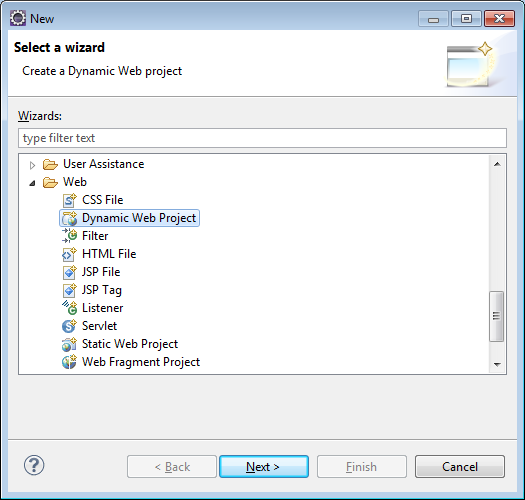
\includegraphics[scale=0.3]{./imagens/apendice_img1.png}}
% \caption[Outra imagem ainda.]
%           {Outra imagem ainda. \textbf{Fonte:} Elaborado pelos autores}
%  \label{fig:ap2:identificador}
%\end{figure}

%\section*{Segunda seção do apêndice 2}


%\par Continuando \ldots na figura Figura~\ref{fig:xml_exemplo} é mostrado um exemplo de XML.

%\begin{figure}[h!]
%\begin{lstlisting}[style=custom_XML]
%<project>
%...
% <dependencies>
%  ...
%  <dependency>
%   <groupId>org.neo4j</groupId>
%   <artifactId>neo4j</artifactId>
%   <version>1.9.4</version>
%  </dependency>
%  ...
% </dependencies>
% ...
%</project>
%\end{lstlisting}  
% \caption[Exemplo de código XML.]
%           {Exemplo de código XML. \textbf{Fonte:} Elaborado pelos autores}
%  \label{fig:xml_exemplo}
%\end{figure}

